% Workflow of the use-conditioned due diligence protocol (revision 1).
% Build from this directory with pdflatex fig_r1_protocol_workflow.tex
% Requires the standalone class and pgf/TikZ.
\documentclass[tikz,border=4pt]{standalone}
\usepackage[T1]{fontenc}
\usepackage{lmodern}
\usetikzlibrary{positioning,arrows.meta,fit,calc}
\definecolor{stagefill}{HTML}{EEF2F7}
\definecolor{stageline}{HTML}{4A6A8C}
\definecolor{briefill}{HTML}{FFF4DE}
\definecolor{briefline}{HTML}{B07C1E}
\definecolor{passc}{HTML}{2E7D32}
\definecolor{failc}{HTML}{C62828}
\definecolor{indc}{HTML}{8D6E00}
\definecolor{actfill}{HTML}{F3F3F3}
\begin{document}
\sffamily
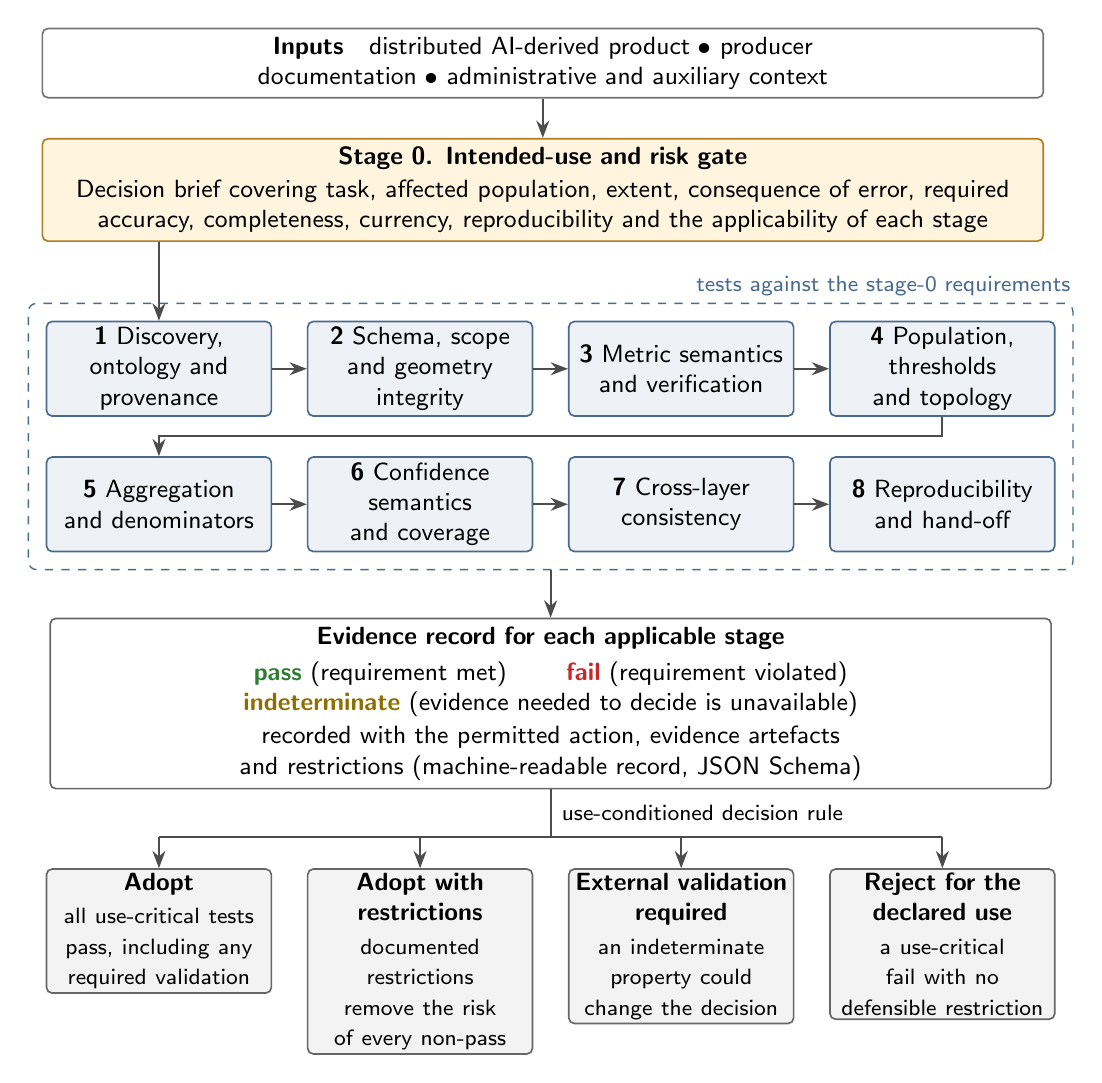
\begin{tikzpicture}[
  font=\sffamily\small,
  every node/.append style={execute at begin node={\hyphenpenalty=10000\exhyphenpenalty=10000}},
  node distance=4mm and 4.4mm,
  stage/.style={draw=stageline, fill=stagefill, rounded corners=2pt, line width=0.6pt,
                minimum height=12mm, text width=27.5mm, align=center, inner sep=1.5pt},
  wide/.style={rounded corners=2pt, line width=0.6pt, text width=125mm, align=center, inner sep=3pt},
  action/.style={draw=black!60, fill=actfill, rounded corners=2pt, line width=0.6pt,
                 minimum height=15mm, text width=27.5mm, align=center, inner sep=1.5pt, anchor=north},
  arr/.style={-{Stealth[length=2.2mm]}, line width=0.7pt, black!70},
]
\node[wide, draw=black!55] (in) {\textbf{Inputs}\quad distributed AI-derived product \textbullet{} producer documentation \textbullet{} administrative and auxiliary context};
\node[wide, draw=briefline, fill=briefill, below=5mm of in] (s0) {\textbf{Stage 0. Intended-use and risk gate}\\[1pt]
  Decision brief covering task, affected population, extent, consequence of error, required accuracy, completeness, currency, reproducibility and the applicability of each stage};

\coordinate (row1) at ($(s0.south west)+(1.5pt,-10mm)$);
\node[stage, anchor=north west] (s1) at (row1) {\textbf{1} Discovery, ontology and provenance};
\node[stage, right=of s1] (s2) {\textbf{2} Schema, scope and geometry integrity};
\node[stage, right=of s2] (s3) {\textbf{3} Metric semantics and verification};
\node[stage, right=of s3] (s4) {\textbf{4} Population, thresholds and topology};
\node[stage, below=5mm of s1] (s5) {\textbf{5} Aggregation and denominators};
\node[stage, right=of s5] (s6) {\textbf{6} Confidence semantics and coverage};
\node[stage, right=of s6] (s7) {\textbf{7} Cross-layer consistency};
\node[stage, right=of s7] (s8) {\textbf{8} Reproducibility and hand-off};

\node[draw=stageline, dashed, rounded corners=3pt, line width=0.5pt, inner sep=2.2mm,
      fit=(s1)(s4)(s5)(s8)] (stages) {};
\node[font=\sffamily\footnotesize, text=stageline, anchor=south east, inner sep=1pt]
      at ($(stages.north east)+(0,0.4mm)$) {tests against the stage-0 requirements};

\node[wide, draw=black!60, below=6mm of stages] (rec) {\textbf{Evidence record for each applicable stage}\\[2pt]
  {\color{passc}\textbf{pass}} (requirement met) \qquad {\color{failc}\textbf{fail}} (requirement violated) \qquad
  {\color{indc}\textbf{indeterminate}} (evidence needed to decide is unavailable)\\[1pt]
  recorded with the permitted action, evidence artefacts and restrictions (machine-readable record, JSON Schema)};

\coordinate (bus) at ($(rec.south)+(0,-6mm)$);
\coordinate (actrow) at ($(bus)+(0,-4mm)$);
\node[action] (a1) at (s1.south |- actrow) {\textbf{Adopt}\\[1pt]\footnotesize all use-critical tests pass, including any required validation};
\node[action] (a2) at (s2.south |- actrow) {\textbf{Adopt with restrictions}\\[1pt]\footnotesize documented restrictions remove the risk of every non-pass};
\node[action] (a3) at (s3.south |- actrow) {\textbf{External validation required}\\[1pt]\footnotesize an indeterminate property could change the decision};
\node[action] (a4) at (s4.south |- actrow) {\textbf{Reject for the declared use}\\[1pt]\footnotesize a use-critical fail with no defensible restriction};

\draw[arr] (in) -- (s0);
\draw[arr] (s0.south -| s1.north) -- (s1.north);
\draw[arr] (s1) -- (s2); \draw[arr] (s2) -- (s3); \draw[arr] (s3) -- (s4);
\draw[arr] (s4.south) -- ++(0,-2.4mm) -| (s5.north);
\draw[arr] (s5) -- (s6); \draw[arr] (s6) -- (s7); \draw[arr] (s7) -- (s8);
\draw[arr] (stages.south) -- (rec.north);
\draw[line width=0.7pt, black!70] (rec.south) -- (bus);
\draw[line width=0.7pt, black!70] (a1.north |- bus) -- (a4.north |- bus);
\foreach \a in {a1,a2,a3,a4} { \draw[arr] (\a.north |- bus) -- (\a.north); }
\node[font=\sffamily\footnotesize, anchor=west, inner sep=1pt] at ($(rec.south)+(1mm,-3mm)$) {use-conditioned decision rule};
\end{tikzpicture}
\end{document}
